\section{The Arm TrustZone Solution}
Arm has developed their \gls{tee} solution which the call ``TrustZone''. When evaluating how Arm’s TrustZone works, we must remember several important distinctions. Firstly, the Arm specifications include several different architectures with several different states. Each Arm architecture and state combination may operate slightly differently in regard to how TrustZone is implemented. This paper will only consider the ARMv8-A architecture running in the AArch64 state. Secondly, hardware manufacturers may choose to implement security in many ways, and with much more flexibility than in Intel platforms. For simplicity’s sake, this paper will only cover standard Arm solutions for TrustZone implementation, provided by Arm's \gls{tfa} and \gls{optee}.
 
Arm \gls{soc} processors create a more absolute separation between the worlds of ``secure'' and ``normal or insecure'' operation than Intel \gls{sgx}. At its highest level this is accomplished using the \gls{scr} ``Non-Secure Bit'' (NS) with 1 meaning non-secure and 0 meaning secure. This is perhaps the most fundamental element that separates Arm's two security worlds. Digging a bit deeper, this separation of worlds is accomplished using three principal technologies on the bus, the \gls{soc} core, and the debug infrastructure. Firstly, the bus interface, called the \gls{amba} \gls{axi}, partitions all of the \gls{soc}’s hardware and software resources by taking advantage of a set of bits. Hardware logic present in this ``TrustZone-enabled AMBA3 AXI'' bus fabric ensures that no ``Secure World'' resources can be accessed by ``Normal World'' components. These bits include AWPROT for write transactions and ARPROT for read transactions where like the NS bit low is Secure and high is Non-secure. Secondly, \gls{soc}s which include cores like the ARMv8-A implement extensions which enable a single physical processor core to safely and efficiently execute code from both the Normal World and the Secure World in a time-sliced fashion. Lastly, the security-aware debug infrastructure controls debug access to the Secure World \cite{ArmBuildingSS}. These three technologies provide a framework or scaffolding on which to build a platform capable of secure computation.

Unlike Intel platforms which refer to their privilege levels as rings, Arm uses ``Exception Levels'' EL0 through EL3 \cite{armfundv8A}. Here EL3 is the highest, most privileged level where as EL0 is the lowest and least privileged level. One important thing to note here is that exceptions (e.g. data aborts, pre-fetch aborts, interrupts) can be taken from the level at which they occur to the same or any higher level, but not a lower level. So, for example, an interrupt occurring in the OS kernel (EL1) can be handled in the kernel or in the secure monitor (EL3), but not in the lower application level (EL0). Practically speaking this means that the user applications running on a system which has not been compromised will not have access to kernel or lower exceptions.

\renewcommand{\arraystretch}{2.5}
\begin{table}[h]
\centering
\begin{tabular}{|l|l|l|}
\hline
\textbf{Privilege Level} & \textbf{Description} & \textbf{Implementation}                                          \\ \hline
EL-0 & Application Privilege Level & Supported by CPU architecture                                                   \\ \hline
EL-1 & Kernel Privilege Level & Supported by CPU architecture                                                   \\ \hline
EL-2 & \makecell[l]{Virtualization Privilege Level \\ (Optional)} & Supported by CPU architecture                                                   \\ \hline
EL-3 & Secure Privilege Level & \makecell[l]{Supported by CPU architecture \\ or a dedicated embedded \\ security processor} \\ \hline
\end{tabular}
\caption{Arm Privilege Level Mapping}
\label{tab:arm_priv_lev_map}
\end{table}


Each exception level manages its own page tables and control registers with the exception of EL0 which is managed by EL1. This is a common practice across architectures where the kernel level mode controls the page table for the applications running on top of it. As we will see, this division is taken advantage of by the ARMv8-A architecture to enable the separation of memory accesses between the Secure World and the Normal World.

\section{Arm Trusted Firmware}
Since 2013, Arm has provided \glsreset{tfa}\gls{tfa} as an open source reference implementation of the firmware required to develop Secure World software for A-Class devices (including ARMv8-A). The \gls{tfa} provides many features including secure device initialization, modular boot flow, trusted boot, and the secure monitor that allows switching between the Normal World and the Secure World. It should be noted that all of this code and documentation is freely available at \url{https://www.trustedfirmware.org/}. The Trusted Firmware Project is a `not for profit' open source project hosted by Linaro Limited (``Linaro'').

Arm Trusted Firmware uses the scaffolding provided by the A-Class devices to implement the key aspects of TrustZone, namely Trusted Boot and the Secure Monitor. There are currently over 30 platforms supported by Trusted Firmware and because the code is open source (BSD 3-clause), porting new platforms can be done by following many of the existing open source examples. Before we explore Arm Trusted Firmware, we must first understand how an Arm platform can be initialized in a secure state, specifically using \gls{tbb}. \gls{tbb} is based on two standards, the Arm Trusted Base System Architecture (TBSA) \cite{Edition2018} and the Arm Trusted Board Boot Requirements (TBBR) \cite{ArmTrustedBoot}. Both of these specifications are client-based solutions and it is likely that server based solutions are in development internally at Arm.

\begin{figure}[ht]
\centering
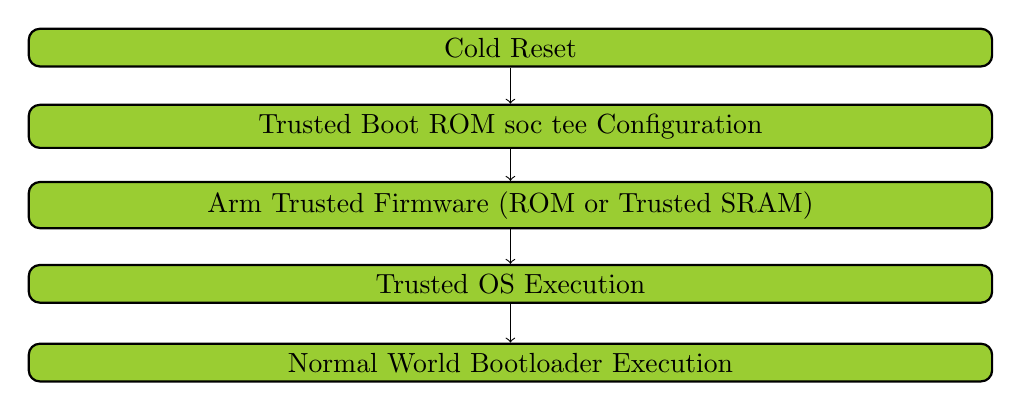
\begin{tikzpicture}[
    block/.style ={rectangle, draw=black, thick, fill=YellowGreen,
          text width=12cm, text centered, rounded corners},
    line/.style ={draw, ->}
]

\node[block] (s1) at (0,0) {Cold Reset};
\node[block, below of = s1] (s3) {Trusted Boot ROM \gls{soc} \gls{tee} Configuration};
\node[block, below of = s3] (s5) {Arm Trusted Firmware (ROM or Trusted SRAM)};
\node[block, below of = s5] (s10) {Trusted OS Execution};
\node[block, below of = s10] (s15) {Normal World Bootloader Execution};

\path [line] (s1) -- (s3);
\path [line] (s3) -- (s5);
\path [line] (s5) -- (s10);
\path [line] (s10) -- (s15);

\end{tikzpicture}

\caption[Arm's Trusted Board Boot]{\textbf{A significantly simplified boot flow for setting up a secure root of trust on an Arm system running Trusted Firmware.} Here we see the boot flow from a cold reset all the way to the Normal World bootloader which may load any untrusted OS kernel.}
\label{fig:tbb-flow}
\end{figure}

As soon as the SoC comes out of power-on-reset, execution happens in integrity protected memory like on-chip Boot ROM or Trusted SRAM. At this stage we have access to a \gls{rotpk} located in one of the \gls{soc}'s \gls{otp} Efuse registers. These keys are usually SHA-256 and the Efuse is burned by the manufacturer to ensure the integrity of the keys. This secure ROM firmware code is often called the Bootloader Stage 1 or BL1, and it is responsible for checking the validity of the \gls{rotpk}. Using this key, BL1 can verify the hash of the next bootloader stage (BL2). The code in BL1 is the only code that must run in EL3, minimizing the amount of initialization code that must run at this critical privilege level.

Once in BL2, the code is executing in Secure World EL2 and the firmware can use the \gls{rotpk} to extract the Trusted World \gls{rotpk} and the Normal World \gls{rotpk}, which are used in turn to validate the Secure World Trusted OS hash as well as the Normal World Untrusted OS hash. All of these keys and hashes are included as extensions to the x.509 standard format, however there is no need for a valid Certified Authority (CA) certificate, as we are verifying the contents of the certificates and not the validity of a certificate issuer. BL2 also does some RAM initialization before it passes off to BL3 where the Secure Monitor is implemented.

This Secure Monitor runs in EL3 and is responsible for loading both the Secure OS as well as the Normal World bootloader (like U-Boot or some UEFI implementation). This Secure Monitor stays resident in memory during the life of the system and will manage the interactions between the Normal and Secure Worlds. All of these stages (BL1 - BL3) of \gls{tbb} are implemented by Arm's \glsreset{tfa}\gls{tfa} reference implementation.

\begin{figure}[ht]
\makebox[\textwidth][c]{\input{tikz/trustzone-overview}
}\caption[Arm TrustZone Example of Normal and Secure World]{\textbf{Secure World implementation using ARM TrustZone.}
The \gls{soc} boots into the Secure World and a monitor is registered which acts as the interface between the Secure and Normal Worlds.
\label{fig:trustzone}}
\end{figure}

Once the Trusted Firmware has initialized the system in a secure state, we have initialized two worlds, the Trusted World and the Normal World. It is perhaps easiest to think about the interaction between these two worlds in much the same way we think about making calls from user mode into kernel mode in Linux systems. In Linux systems, we take advantage of system calls (syscall) to bridge a trust boundary between the kernel's concerns like interacting with a network card and the user application's concerns like displaying a web page. At no point in this interaction should the user application code have access to the network card's buffers, however the kernel is able to read and write these buffers and mediate the flow of data to/from the client application. This ``guarded'' flow of data is similar to how memory in the Secure World is kept separate from the Normal World using an instruction which generates an exception called a Secure Monitor Call (SMC).

\section{TrustZone Attestation}